\section{Hydroponicsystemcontroller}

Das Ziel dieses Projektes ist es einen Regelkreis für eine sich selbst regulierende, indoor hydroponische Pflanzenzucht zu bauen. Zu betrachtende Faktoren hierbei sind Temperatur (des Wassers, als auch eventurell der Lufttemperatur), die Düngerkonzentration im Wasser, sowie der pH-Wert der Lösung. Um das Problem der Düngerkonzentration in einem für uns umsetzbaren Rahmen zu halten, wird die relative Ionenkonzentration untereinander, während eines Wachstumszyklus, vorersts als konstant angenommen. Die Düngerkonzentration kann somit als direkt proportional zur elektrischen Leitfähigkeit (EC) der Flüssigkeit modeliert werden.\\
Fällt einer der Ist-Werte unter den Soll-Zustand, so wird mittels dem selbstgebaute rotary-vane-pump gegengestäuert (Dünger oder pH-UP/-Down).\\
Aus den Temperatur-, EC- und pH-Wert-Daten soll dann ebenso ein Modell für die Löslichkeit der Düngersalze, bzw. die zeitabhängige Veränderung des EC-Wertes bei Zugabe des Düngers, erstellt werden.\\
\\
\textbf{Bonus-Task:}
Ursprünglich wollten wir die Konzentration der einzelnen, gelösten Ionen bestimmen. Da diese Form der Analyse aber zum einen sehr aufwendig, und schlimmer noch, extrem kostenintensiv ist, scheint Spektroskopie im IR-Bereich für unsere Zwecke am hilfreichsten zu sein(Das Verhältnis der Hauptkomponenten unseres Düngers lässt sich durch IR-Spektroskopie abschätzen). Da der zusätzliche Bau eines Spektroskops zu viel für den Rahmen dieses Projektes wäre, könnten wir, falls möglich, einen komerziellen Spektrographen zu Vorführungszwecken benutzen und die Daten in unsere Modellierung mit ein beziehen. Dies wäre allerdings nur als Bonus zum Projekt gedacht und gehört nicht zum eigentlichen Projektvorschlag.

\section*{Fragestellung}

\section*{Projektaufbau}

\begin{figure}[H]
    \centering
    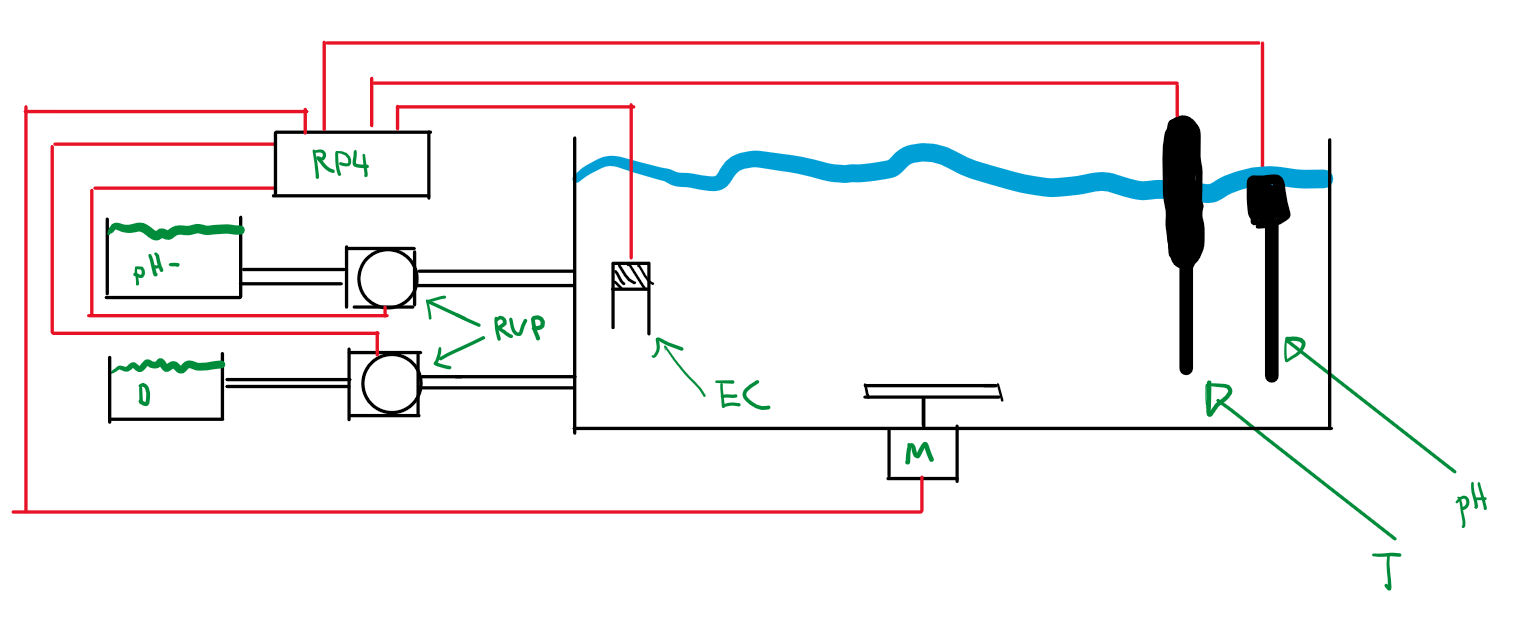
\includegraphics[width=\linewidth]{skizze.png}
    \caption{
        Skizze des Coil-Winders und der magnetischen Spannvorrichtung.
        \textbf{pH-}: (pH-)-Lösung; 
        \textbf{D}: Dünger-Lösung; 
        \textbf{RVP}: Rotary-Vane-Pump; 
        \textbf{EC}: Leitfähigkeitssensor; 
        \textbf{M}: Rührmotor; 
        \textbf{RP4}: Raspberry Pi 4; 
        \textbf{T}: Thermometer; 
        \textbf{pH}: ph-Messgerät;
    }
\end{figure}

\section*{Physikalische Anforderungen}
\begin{enumerate}
    \item Stuff
\end{enumerate}


\section*{Komponenten und Kosten}
\begin{table}[H]
    \centering
    \caption{
        Skizze
    }
    \begin{tabular}{| c | c |}
        \hline
        Komponente &  Kosten / \euro{}\\
        \hline
        Ding & 15 - 30  \\
        \hline
        \hline
        Summe & 110 - 225  \\
        \hline
    \end{tabular}
    \label{tab:Komponenten}
\end{table}


\section*{Software}
\begin{enumerate}
    \item Code
\end{enumerate}

\section*{Aufwandsabschätzung}
\begin{table}[H]
    \centering
    \caption{
        Skizze
    }
    \begin{tabular}{| c | c |}
        \hline
        Arbeitspaket &  Aufwand / h\\
        \hline
        Arbeit & 30 - 45  \\
        \hline
        \hline
        Summe & 120 - 230  \\
        \hline
    \end{tabular}
    \label{tab:Aufwand}
\end{table}